%% USEFUL LINKS:
%% -------------
%%
%% - UiO LaTeX guides:          https://www.mn.uio.no/ifi/tjenester/it/hjelp/latex/
%% - Mathematics:               https://en.wikibooks.org/wiki/LaTeX/Mathematics
%% - Physics:                   https://ctan.uib.no/macros/latex/contrib/physics/physics.pdf
%% - Basics of Tikz:            https://en.wikibooks.org/wiki/LaTeX/PGF/Tikz
%% - All the colors!            https://en.wikibooks.org/wiki/LaTeX/Colors
%% - How to make tables:        https://en.wikibooks.org/wiki/LaTeX/Tables
%% - Code listing styles:       https://en.wikibooks.org/wiki/LaTeX/Source_Code_Listings
%% - \includegraphics           https://en.wikibooks.org/wiki/LaTeX/Importing_Graphics
%% - Learn more about figures:  https://en.wikibooks.org/wiki/LaTeX/Floats,_Figures_and_Captions
%% - Automagic bibliography:    https://en.wikibooks.org/wiki/LaTeX/Bibliography_Management  (this one is kinda difficult the first time)
%%
%%                              (This document is of class "revtex4-1", the REVTeX Guide explains how the class works)
%%   REVTeX Guide:              http://www.physics.csbsju.edu/370/papers/Journal_Style_Manuals/auguide4-1.pdf
%%
%% COMPILING THE .pdf FILE IN THE LINUX IN THE TERMINAL
%% ----------------------------------------------------
%%
%% [terminal]$ pdflatex report_example.tex
%%
%% Run the command twice, always.
%%
%% When using references, footnotes, etc. you should run the following chain of commands:
%%
%% [terminal]$ pdflatex report_example.tex
%% [terminal]$ bibtex report_example
%% [terminal]$ pdflatex report_example.tex
%% [terminal]$ pdflatex report_example.tex
%%
%% This series of commands can of course be gathered into a single-line command:
%% [terminal]$ pdflatex report_example.tex && bibtex report_example.aux && pdflatex report_example.tex && pdflatex report_example.tex
%%
%% ----------------------------------------------------


\documentclass[english,notitlepage,reprint,nofootinbib]{revtex4-1}  % defines the basic parameters of the document
%,biblatex

% Allows special characters (including æøå)
\usepackage[utf8]{inputenc}

%\usepackage[
%backend=biber,
%style=alphabetic,
%sorting=none
%]{biblatex}
\usepackage{physics,amssymb}  % mathematical symbols (physics imports amsmath)
\include{amsmath}
\usepackage{graphicx}         % include graphics such as plots
\usepackage{xcolor}           % set colors
\usepackage{hyperref}         % automagic cross-referencing
\usepackage{listings}         % display code
\usepackage{subfigure}        % imports a lot of cool and useful figure commands
\usepackage{float}
%\usepackage[section]{placeins}
\usepackage{algorithm}
\usepackage[noend]{algpseudocode}
\usepackage{subfigure}
\usepackage{tikz}
\usepackage{xcolor}
\usetikzlibrary{quantikz}
\usepackage{pgf}
\usepackage{enumerate}

% defines the color of hyperref objects
% Blending two colors:  blue!80!black  =  80% blue and 20% black
\hypersetup{ % this is just my personal choice, feel free to change things
    colorlinks,
    linkcolor={red!50!black},
    citecolor={blue!50!black},
    urlcolor={blue!80!black}}

\usepackage{algorithm}
\usepackage[noend]{algpseudocode}
\usepackage{algpseudocode}
\bibliographystyle{apsrev4-2}



%\addbibresource{references.bib} % Imports bib file
% ===========================================
                       % self-explanatory
\begin{document}
\title{Regression analysis and resampling methods}  % self-explanatory
\author{Erlend Kristensen, Mathias Mellemstuen, Magnus Selmer-Anderssen Kråkenes} % self-explanatory
\date{\today}      


\noaffiliation                            % ignore this, but keep it.

%This is how we create an abstract section.
\begin{abstract}
    In this report we have looked at the effectiveness of the OLS implementation, as well as proven that using resampling methods will allow us to both get a better model with lower amount of errors and also reduce the chances of overfitting our model. Different resampling methods were proven to be effective in each their perspective, either when it comes to making a highly precise model, where Ridge regression combined with bootstrapping was the best, or a model that is quicker to compute, where Lasso regression combined with Cross-validation proved useful.
\end{abstract}
\maketitle


% ===========================================

\section{Introduction}
\label{sec:INTRODUCTION}
Regression analysis is a powerful process used for estimating the relationship between different variables. This project will look at using different methods of polynomial regression for creating a model for estimating terrain. We will implement and compare the result of using \textit{ordinary least square} (OLS), \textit{lasso} and \textit{ridge regression}. These methods will first be tested with our own generated sample data using the \textit{Franke function}. Then we will transition over to testing this on real digital terrain data.

We will introduce the necessary methods and theory to solve the problem in section \ref{sec:METHODS}. Then the results will be presented in section \ref{sec: FIGURES} and discussed further in section \ref{sec:DISCUSSION}. We will then have a overall conclusion in section \ref{sec:CONCLUSION}.
\section{THEORY AND METHODS}
\label{sec:METHODS}


\subsection{Expectation values and variances}
\label{subsec: Example}
A basis for ordinary least squares regression (OLS) is the assumption that our data, y, can be described by an existing continuous function f(x) and an error. In our case we assume a normally distributed error $\epsilon \sim$  N(0, $\sigma^2$), which gives us 
\begin{align}
    y = f(x) + \epsilon
\end{align} \label{1}
The function f(x) can be approximated as a matrix X multiplied with a vector $\beta$, that is
\begin{align}
    \bar{y} = X\beta
\end{align}
where X is the design matrix, which is based on our model and will vary depending on how many polynomials we use (see appendix \ref{sec:NOTATION}), and $\beta$ is an unknown parameter which is found by minimizing $(y - \bar{y})^2$. For a given element $y_{i}$, we can calculate the expectation value by summing the expectation values of $X_{i,*}\beta$ and $\epsilon$. As the input x is predetermined, X$\beta$ is a deterministic value, so the expected value for a given i is $X_{i,*}\beta$. Since $\epsilon$ is normally distributed, the expected value of $\epsilon_{i}$ is the mean value, which we assume is 0. The expected value of $y_{i}$ is thus 
\begin{align}
    \mathbb{E}(y_{i}) = X_{i,*}\beta,
\end{align}
 This is the predicted value of y when using the input values of the row i in the design matrix. When predicting there will, unless the model that is used is perfect, always be some degree of error in the prediction. That is, for a given set of variables, the output y will vary around a mean, which is the expected value $\mathbb{E}(y_{i})$. It is therefore important to provide some sort of error estimation along with the prediction. The variance is a measure of the spread around the mean, and can, in addition to being informational by itself, also be used in the analysis of the bias-variance trade off and to calculate the standard deviation. We can calculate the variance of a predicted value $y_{i}$ by squaring the difference between the real value of $y_{i}$ and our approximation of $y_{i}$. We end up with
\begin{align}
    Var(y_{i}) = \sigma^2,
\end{align}
Since $X\beta$ is deterministic it has no effect on the distribution of y. As the error $\epsilon$ is normally distributed, and because this is the only stochastic variable affecting y, we have that y is normally distributed with a mean X$\beta$ and a variance $\sigma^2$.\\
%beta variable
The parameter $\beta$ is an estimator of the regression coefficients. That is, $\beta$ describes the effect each feature has on the output. Following the process of minimizing the cost function of $\beta$ given in the lecture notes from week 34, we have the optimal parameter $\hat{\beta}$
\begin{align}
    \hat{\beta} = (X^TX)^{-1}X^Ty
\end{align}
Calculating the expected value of $\hat{\beta}$ gives us
\begin{align}
    \mathbb{E}(\hat{\beta}) = \beta
\end{align}
The fact that the expected value of the optimal parameter $\beta$ equals the real value of $\beta$ means that $\beta$ is an unbiased parameter. %Explain?
The variance of the optimal parameter $\hat{\beta}$ is 
\begin{align}
    Var(\hat{\beta}) = \sigma^2(X^TX)^{-1}
\end{align}
The variance of $\hat{\beta}$ is useful as it allows us to create confidence intervals for $\hat{\beta}$. Calculating y using the lower and upper values of the confidence interval gives us a prediction interval for y with a certainty determined by the amount of standard errors used for the confidence interval. 

\subsection{Methods}\label{subsec: METHODS}
To be able to test the functionality of our OLS, we will need a good function to approximate and will therefore use the Franke function.
The Franke Function is a 2-dimensional exponential function (as seen in appendix \ref{sec:FUNCTIONS}). Because of its complexity, the function is widely used as a test function for interpolation and fitting problems. However, it is not enough to simply use this function by itself, since we need a way to measure how well our OLS works. To do this, we will use a measurement of error called \textit{the mean squared error} (MSE).

MSE is measuring the average of the errors squared. The MSE tells us how close the estimated value is to the correct value. It tells us how accurate our estimation is. MSE can be defined as
\begin{align}
    MSE(y, \Tilde{y}) = \frac{1}{n} \sum_{i = 0}^{n - 1}(y_{i} - \Tilde{y}_{i})^2
\end{align}
Further on, we will also use the $R^2$ as a measure of performance.

The $R^2$ score is a measure of how much of the variance in the dependent variable which is explained by the independent variables. That is, it explains how much of the spread in the output which can be explained by our input. The $R^2$ score is given as the percentage, or fraction, of the variability in the output which can be explained by our model. It is defined as 
\begin{align}
    R^2 (y, \Tilde{y}) = 1 - \frac{ \sum_{i=0}^{n-1} (y_{i} - \Tilde{y_{i}})^2} {\sum_{i=0}^{n-1} (y_{i} - \bar{y_{i}})^2}
\end{align}
A high $R^2$ score indicates a good model. In machine learning the $R^2$ score is used as a measure of how well the model will predict future samples.

\section{Implementation}\label{sec:IMPLEMENTATION}

\subsection{OLS on the Franke function}\label{subsec:OLS}
We now move on to the implementation of OLS on the Franke function as discussed above. We start by generating our own data set $x,y \in [0,1]$ and transforming them to get the $2D$ data that we need. When we input this data into the Franke function, we add slight noise to it so it better simulates real life data, which is most often not uniformly distributed. We will also split our data sets into a training set and test set, where the training set consists of $80 \%$ of the data, and the test set has the rest. This is to ensure that we don't get a model that is over-fit, but instead more generalized. We do this by training on the training set, and testing the trained model with both our training and test set to see if they both perform well. We will then proceed with scaling the data to ensure that unreasonable high or low peaks in the data are smoothed out, so the data is more similar to real life expected data. The method we used for scaling is the so called \textit{feature standardization}, which makes the value of each feature in the data have a mean of $0$ and a variance of $1$. This normalization method will remove all massive outliers, which is beneficial for making our data set realistic.
% Suggested addition: Scaling our data is not strictly necessary at this moment, as our input variables are already scaled, and our data, despite the added noise, contains no major outliers. Nevertheless, we choose to scale our data as this has little effect on the result, while also allowing us to reuse the code for the real data set later. 

We then proceed with calculating the MSE and $R^2$ scores for both training and test data. Results can be found bellow in section (\ref{sec: FIGURES}).

\subsection{Resampling Techniques}\label{subsec:RESAMPLING}
When creating our design matrix $X$, we choose the number of polynomials we wish to use. As we increase the number of polynomials, the results will improve. However, as said earlier with over-fitting, there will be a certain limit where more polynomials will give worse results. It is therefore useful to find which polynomial degree gives the least amount of error. To do this, we first calculated the MSE of our test and training data, to see how it changes when we increase our polynomials. Knowing what to expect, we then proceed with a resampling technique called \textit{bootstrapping}.
\\
Bootstrapping is a method where we randomly resample our data set $N$ number of times, and calculate the estimated value for each resample. This way, we ensure that the results we get are within what is to be expected, and not just a fluke. When bootstrapping, we will focus on 
\begin{align}
    \mathbb{E}[(\textbf{y} - \mathbf{\tilde y})^2] = (Bias[\tilde y])^2 + var[\tilde f] + \sigma^2
\end{align}
which can be found by optimizing the MSE via the \textit{cost function}
\begin{align}
    C(\mathbf{X}, \mathbf{\beta}) = \frac{1}{n} \sum_{i = 0}^{n - 1} (y_i - \tilde y_i)^2 = \mathbb{E}[(\textbf{y} - \mathbf{\tilde y})^2] 
\end{align}

to do this, we have to keep in mind that the variance of $\mathbf{y}$ and $\mathbf{\epsilon}$ are both equal to $\sigma^2$ (see appendix \ref{sec:NOTATION} for further proof).
This is called the \textit{Bias-variance tradeoff}. The reason we want to study both the bias and variance is to see for which polynomials our model overfits and which polynomials underfit. High bias is a sign of underfitting and high variance is a sign of overfitting.
\\
We have now established that we can use the bootstrapping to find both the bias and variance of our OLS. We will then do this to further investigate how the change in polynomials affects our results.
\\
\\
To further test this, we use another resampling method called \textit{Cross-validation}, and compare it to the result of our bootstrapping. We implement the so called \textit{k-fold} algorithm, which starts by shuffling the data set and divides it into k groups, where one of the groups is taken as a test set and the rest are training sets. Then it fits a model using the training set and tests with the test set. We will do this for 5 to 10 different folds. The reason we want to try Cross-vaildation is because it is a much faster resampling technique, and if it performs similar to bootstrapping, it would be a better choice performance wise.

\subsection{Lasso and Ridge regression}\label{subsec:LASSO_RIDGE}
So far we have calculated expectation values using OLS, but there are other methods as well which may give better results. We therefore repeat the previous steps, now using the ridge regression and lasso methods. Both of these methods take an extra variable, $\lambda$ and $\alpha$ respectively, which work as tuning parameters. $\lambda$ and $\alpha$ are called hyperparameters, and they allow us to reduce the effect of, or completely remove, less relevant features in our model. These methods could therefore, for the right values of $\lambda$ or $\alpha$, give us a better MSE than what was achieved using OLS. To look for good values for our hyperparameters we simply run our ridge regression and lasso algorithms with different values of $\lambda$ and $\alpha$ respectively, with values ranging from very low, $10^{-3}$, to quite high, $10^{1}$. Analyzing the results will show us which values of $\lambda$ and $\alpha$ that give the best fit for their respective methods, and whether or not the methods are effective in reducing the MSE. 

\section{FIGURES AND RESULTS}\label{sec: FIGURES}

\begin{figure*}
    \centering
    \subfloat{{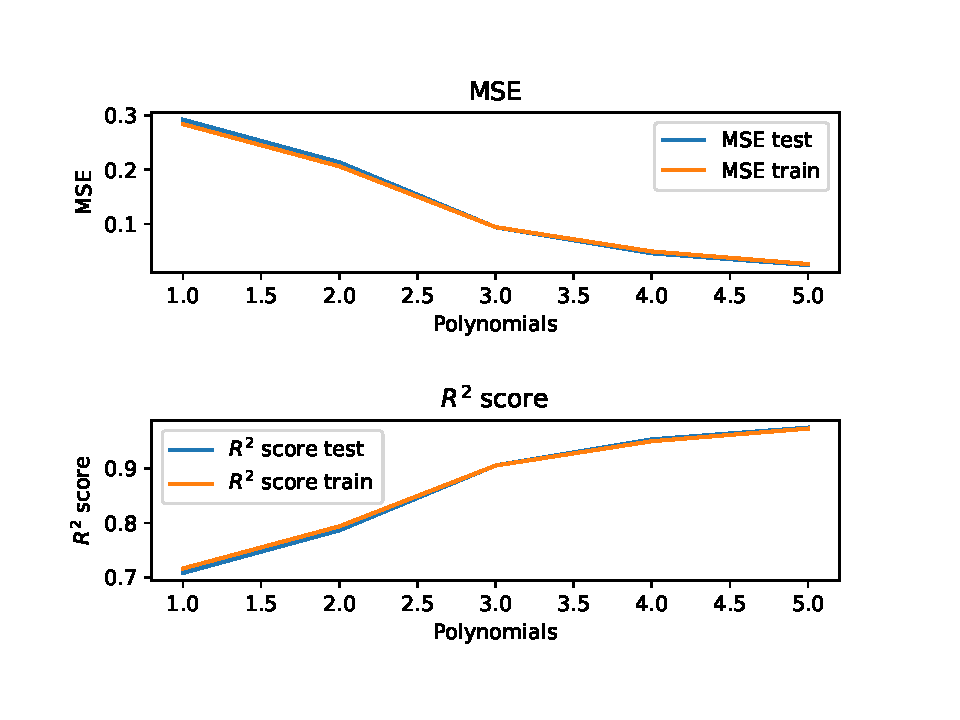
\includegraphics[width=0.45\textwidth]{OLS.pdf} }}%
    \qquad
    \subfloat{{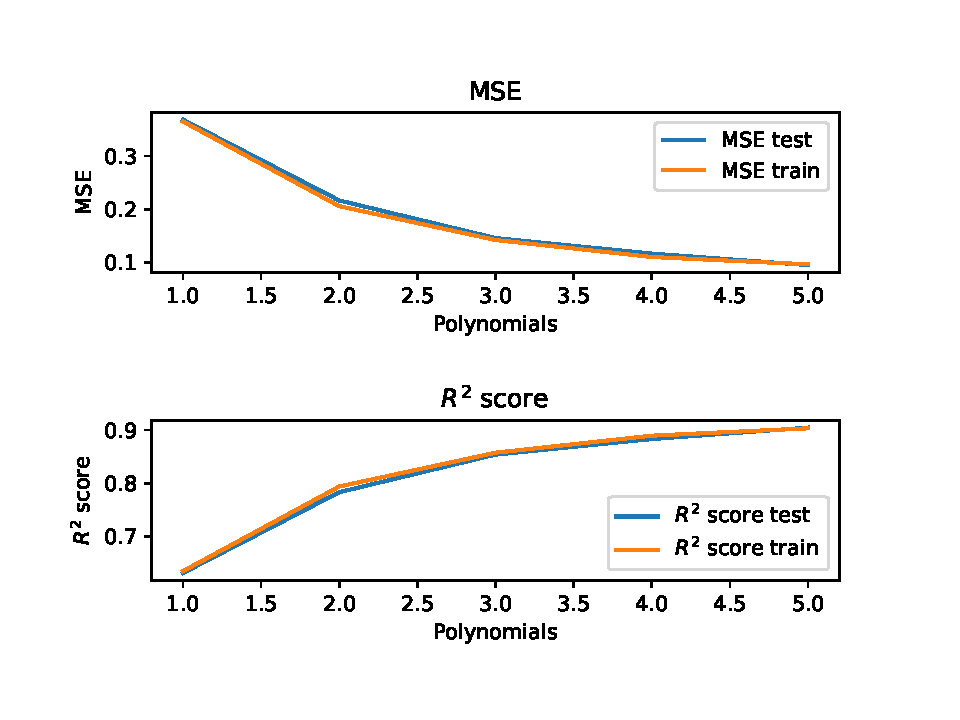
\includegraphics[width=0.45\textwidth]{OLS_Real.pdf} }}%
    \caption{Figures showing the change in MSE and $R^2$ when using $1$ to $5$ degrees of polynomials. The left picture was made with synthetic data, right picture was made using real data.
    The top picture of the plots is our MSE and the bottom picture is our $R^2$ score. The plots show the change for both the training and test data. 
    The synthetic data used was $x,y \in [0,1]$ with an interval of $0.01$, so $100 \times 100$ data points in total, and a maximum noise of $0.01$. The real data used was a $100 \times 100$ cut-out of the image SRTM\_data\_Norway\_1.tif.}
    \label{fig: OLS}
\end{figure*}

\begin{figure*}
    \centering
    \subfloat{{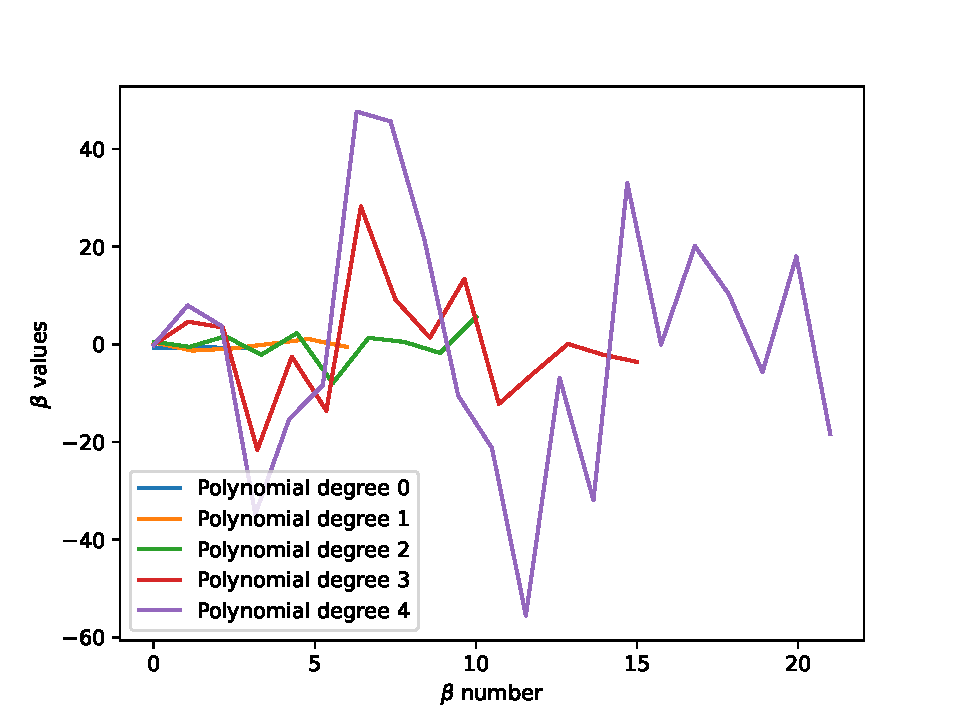
\includegraphics[width=0.45\textwidth]{Beta_values.pdf} }}%
    \qquad
    \subfloat{{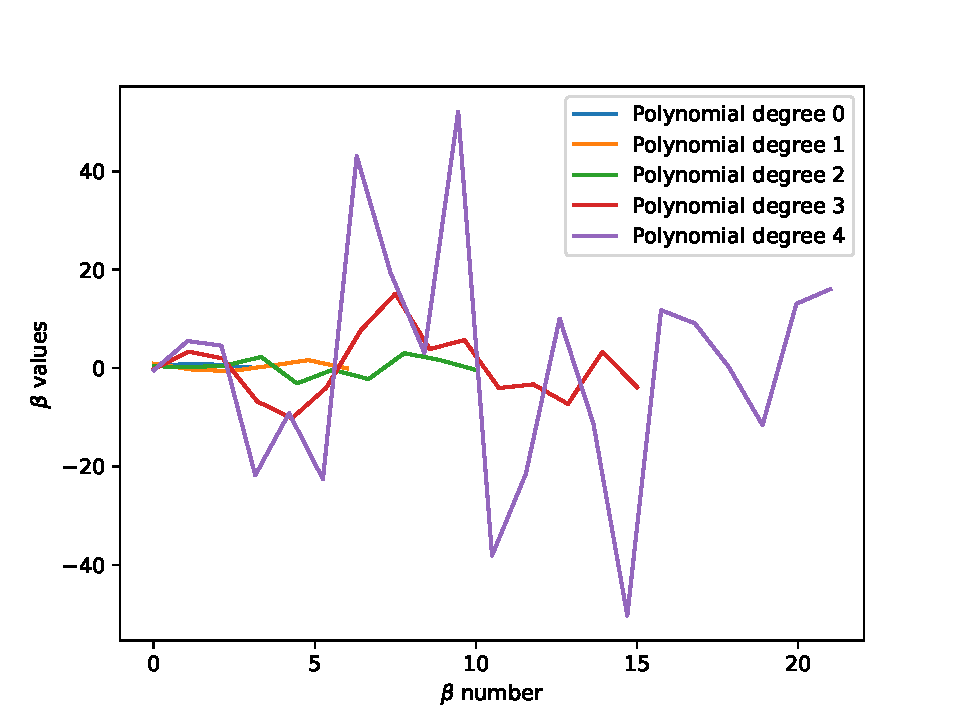
\includegraphics[width=0.45\textwidth]{Beta_values_Real.pdf} }}%
    \caption{Figures showing the $\beta$ values when using $1$ to $5$ degrees of polynomials. The left picture was made with synthetic data, right picture was made using real data.
    The synthetic data used was $x,y \in [0,1]$ with an interval of $0.01$, so $100 \times 100$ data points in total, and a maximum noise of $0.01$. The real data used was a $100 \times 100$ cut-out of the image SRTM\_data\_Norway\_1.tif.}
    \label{fig: BETA_VALUES}
\end{figure*}

\begin{figure*}
    \centering
    \subfloat{{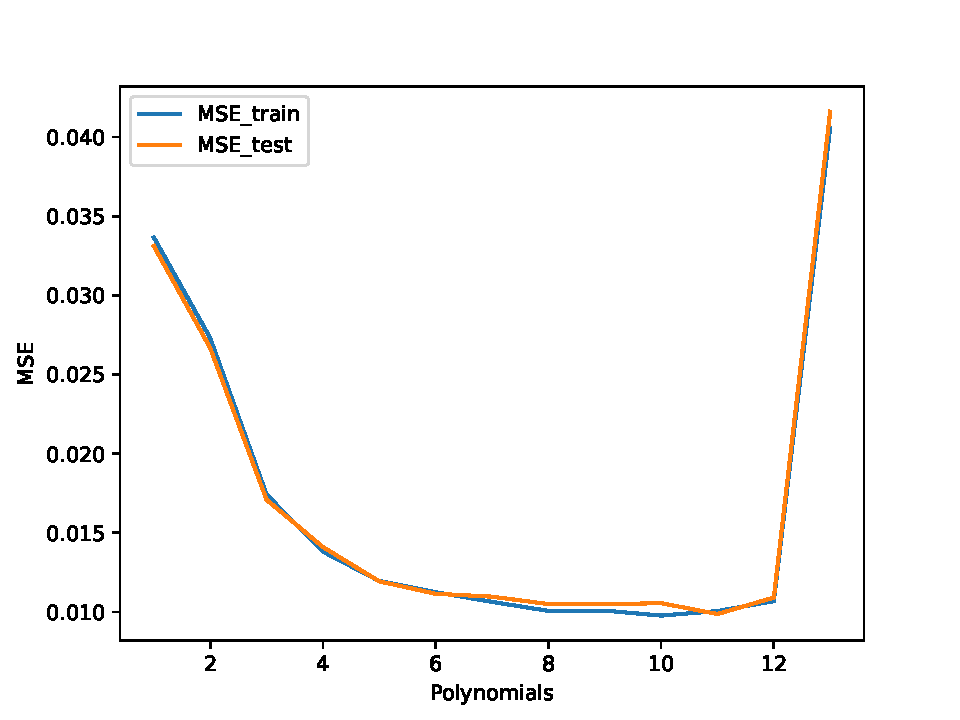
\includegraphics[width=0.45\textwidth]{MSE_test_train.pdf} }}%
    \qquad
    \subfloat{{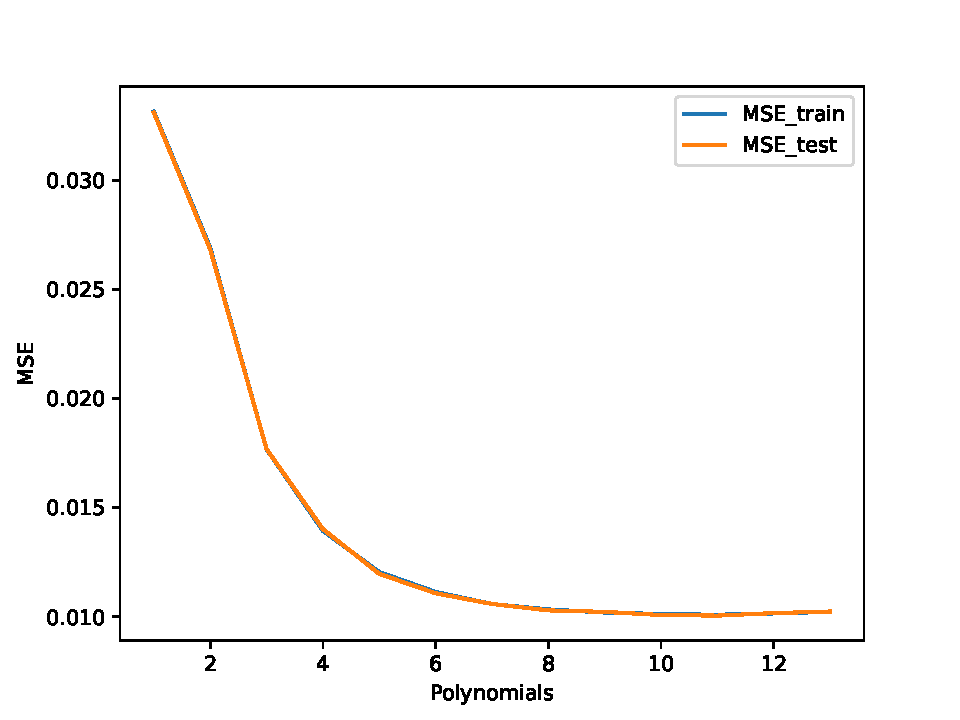
\includegraphics[width=0.45\textwidth]{MSE_test_train_Real.pdf} }}%
    \caption{Figure showing the changes MSE when using $1$ to $13$ degrees of polynomials.}
    The data used for the left picture was $x,y \in [0,1]$ with an interval of $0.01$, so $100 \times 100$ data points in total, and a maximum noise of $0.01$. The right picture used our real data, so $100 \times 100$ data points.
    \label{fig: MSE}
\end{figure*}


\begin{figure*}
    \centering
    \subfloat{{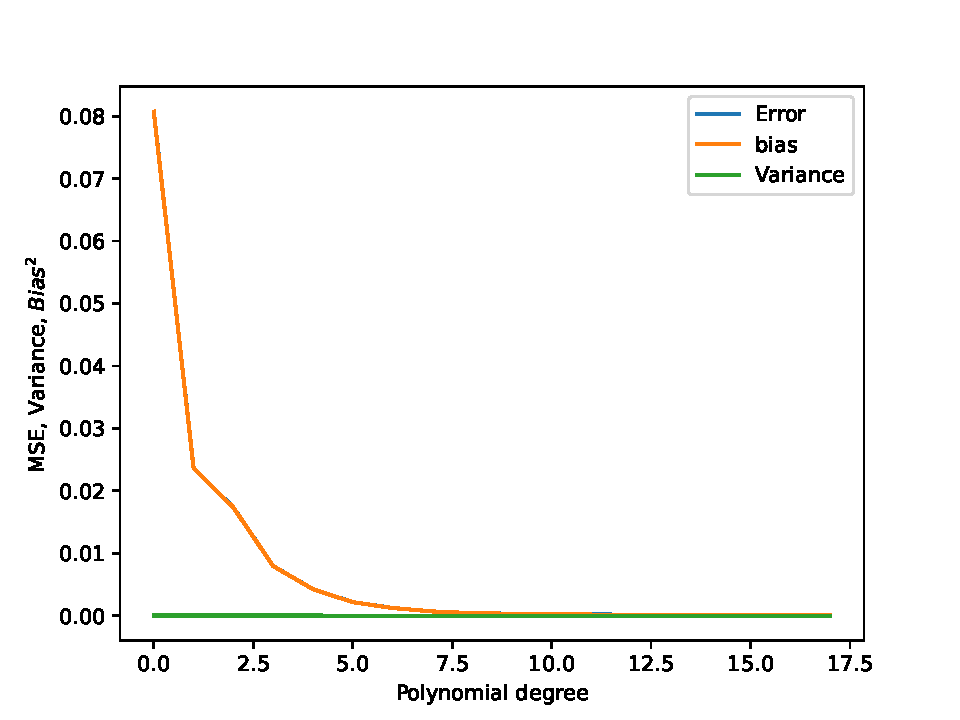
\includegraphics[width=0.45\textwidth]{Part_C_test_18_deg.pdf} }}%
    \qquad
    \subfloat{{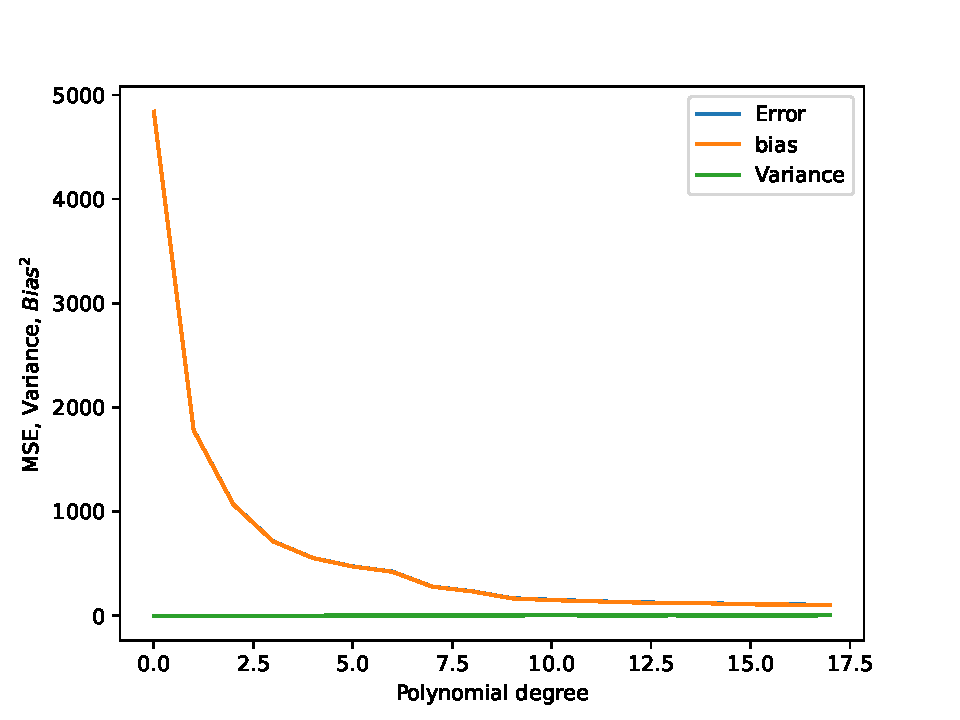
\includegraphics[width=0.45\textwidth]{PartC_real_18_deg.pdf} }}%
    \subfloat{{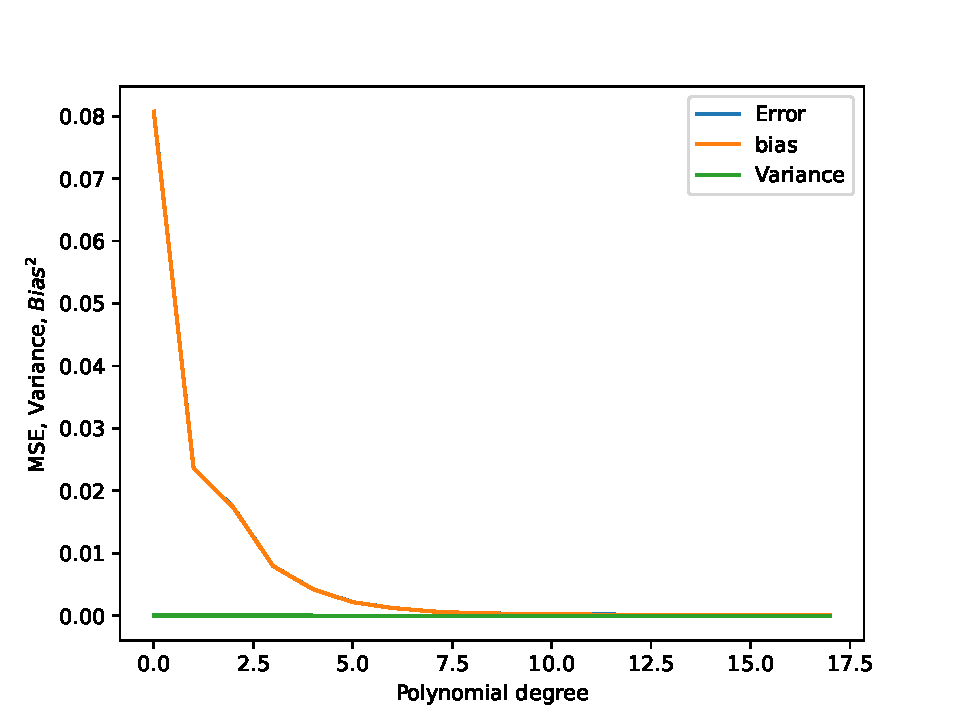
\includegraphics[width=0.45\textwidth]{Part_C_test_18_deg_100_n.pdf} }}%
    \qquad
    \subfloat{{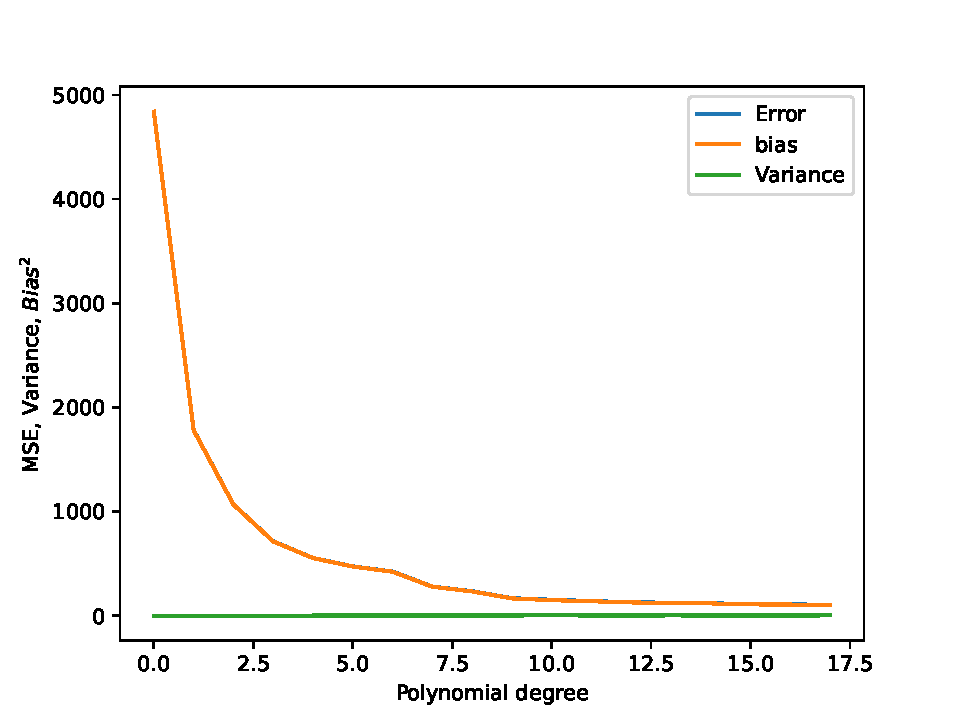
\includegraphics[width=0.45\textwidth]{Part_C_real_18_deg_100_n.pdf} }}%
    \caption{Figures showing the change in bias, variance and MSE when using $1$ to $18$ degrees of polynomials with bootstrapping.}
    The data used for the left picture was $x,y \in [0,1]$ with an interval of $0.01$, so $100 \times 100$ data points in total, and a maximum noise of $0.01$. We also resampled the data $500$ times (top picture) and $100$ times (bottom picture) when bootstrapping. The right pictures used our real data, so $100 \times 100$ data points.
    \label{fig: BOOTSTRAP}
\end{figure*}


\begin{figure*}
    \centering
    \subfloat{{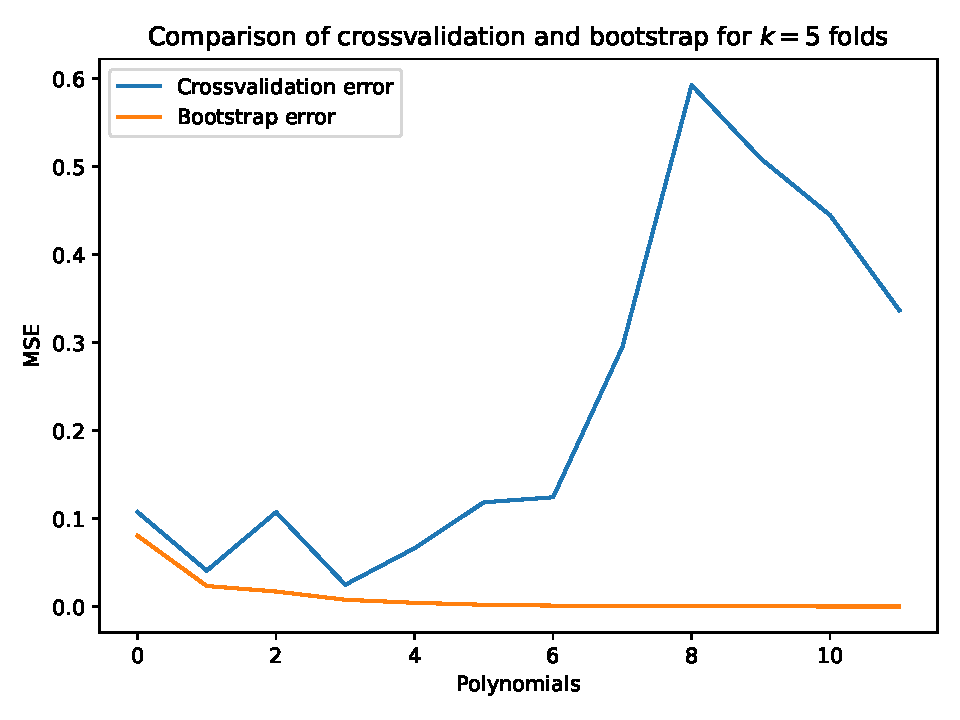
\includegraphics[width=0.45\textwidth]{KFOLD_5.pdf} }}%
    \qquad
    \subfloat{{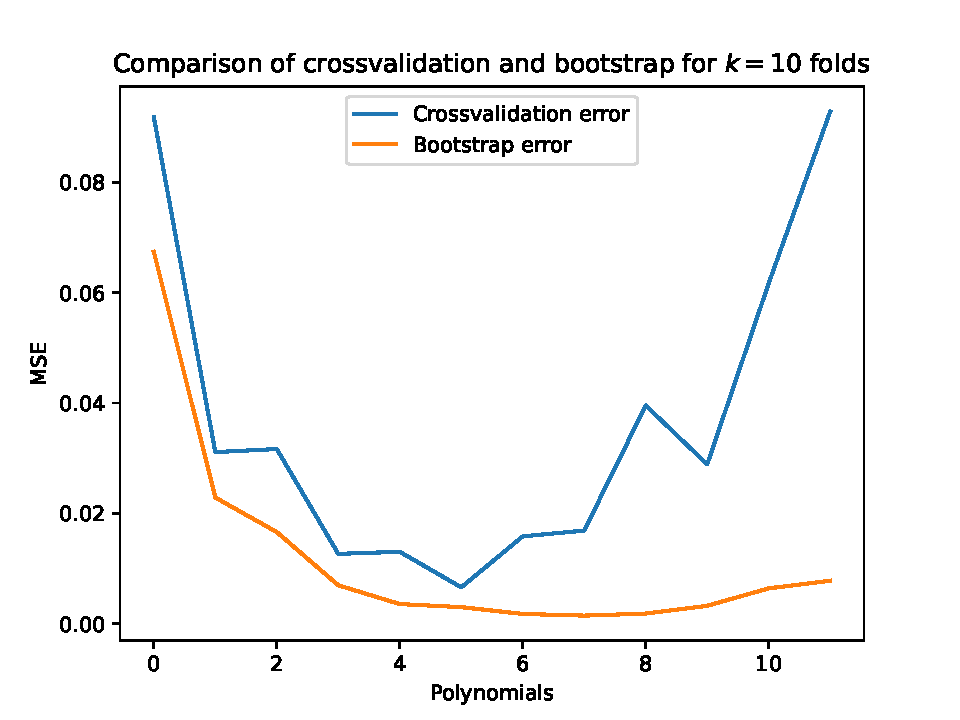
\includegraphics[width=0.45\textwidth]{KFOLD_10.pdf} }}%
    \subfloat{{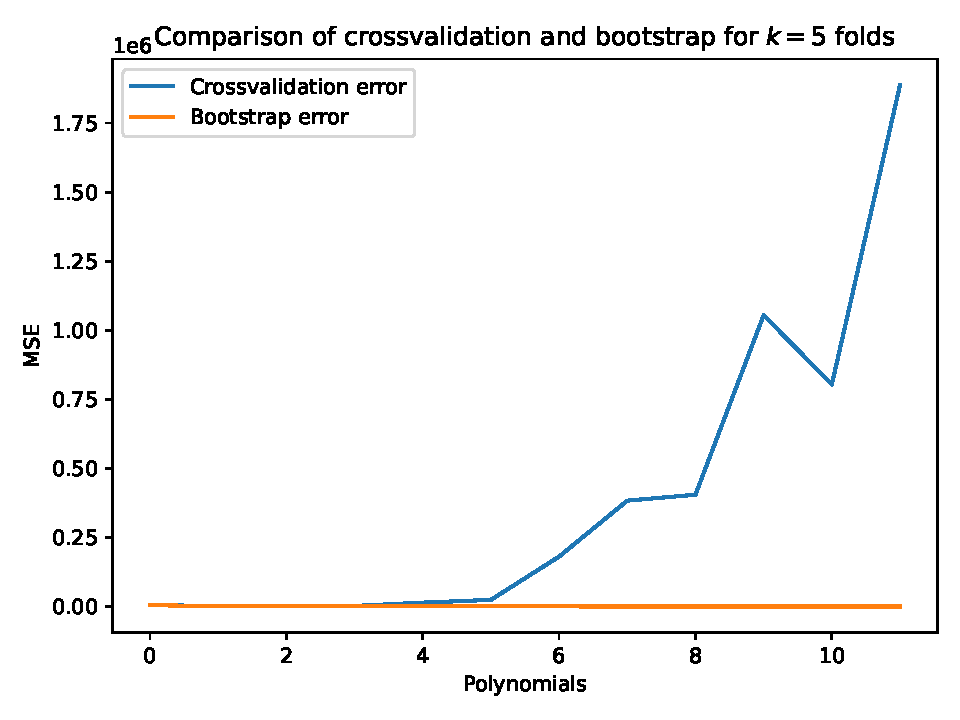
\includegraphics[width=0.45\textwidth]{KFOLD_Real_5.pdf} }}%
    \qquad
    \subfloat{{\includegraphics[width=0.45\textwidth]{KFOLD_Real_10.pdf} }}%
    \caption{Figures showing the change in MSE using $1$ to $11$ degrees of polynomials for bootstrap and cross validation. The left picture was made using $5$ folds and the right picture was made using $10$ folds.
    The data used for the top pictures were $x,y \in [0,1]$ with an interval of $0.01$ and the bottom pictures used the real data, so $100 \times 100$ data points in total for each, and a maximum noise of $0.01$ for the synthetic data. We resampled the data 500 times when bootstrapping.}
    \label{fig:KFOLD}
\end{figure*}


\begin{figure*}
    \centering
    \subfloat{{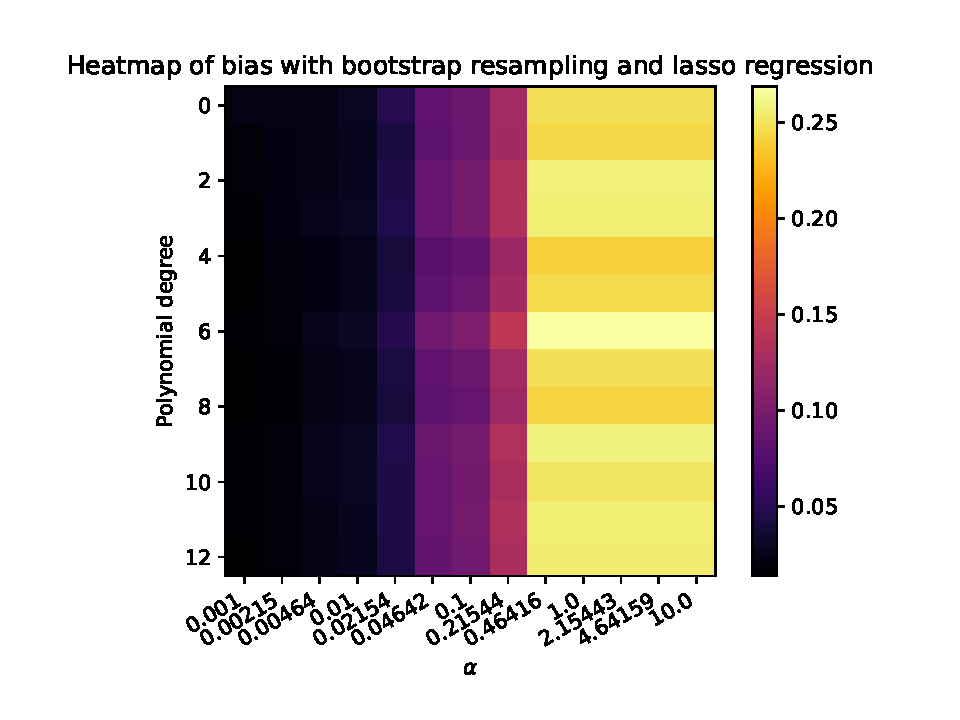
\includegraphics[width=0.45\textwidth]{Heatmap_Bias_Bootstrap_Lasso.pdf} }}%
    \qquad
    \subfloat{{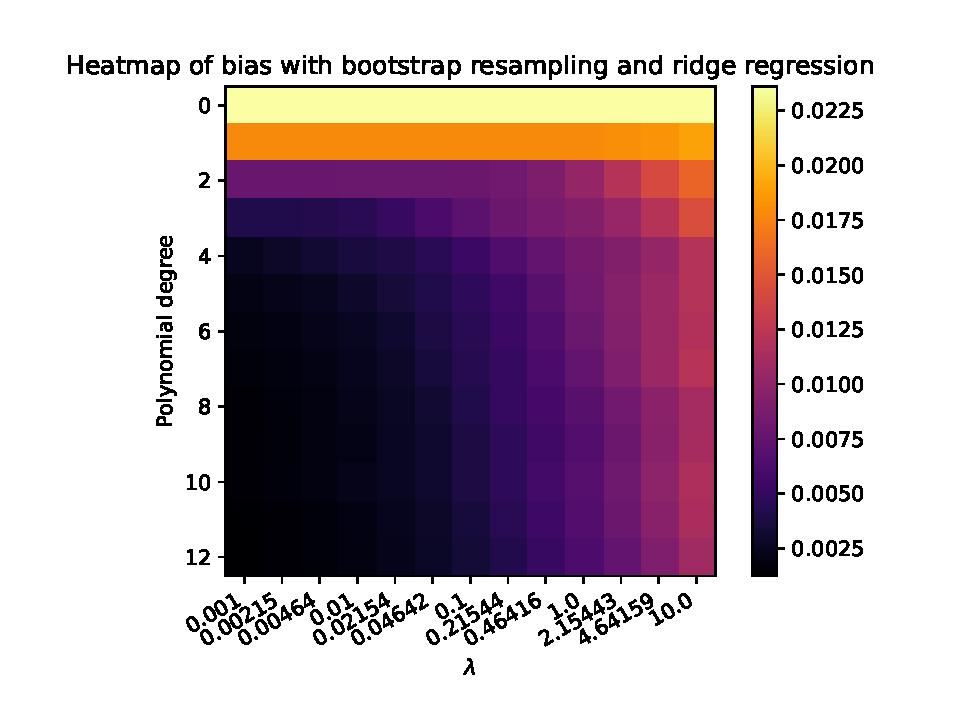
\includegraphics[width=0.45\textwidth]{Heatmap_Bias_Bootstrap_Ridge.pdf} }}%
    \subfloat{{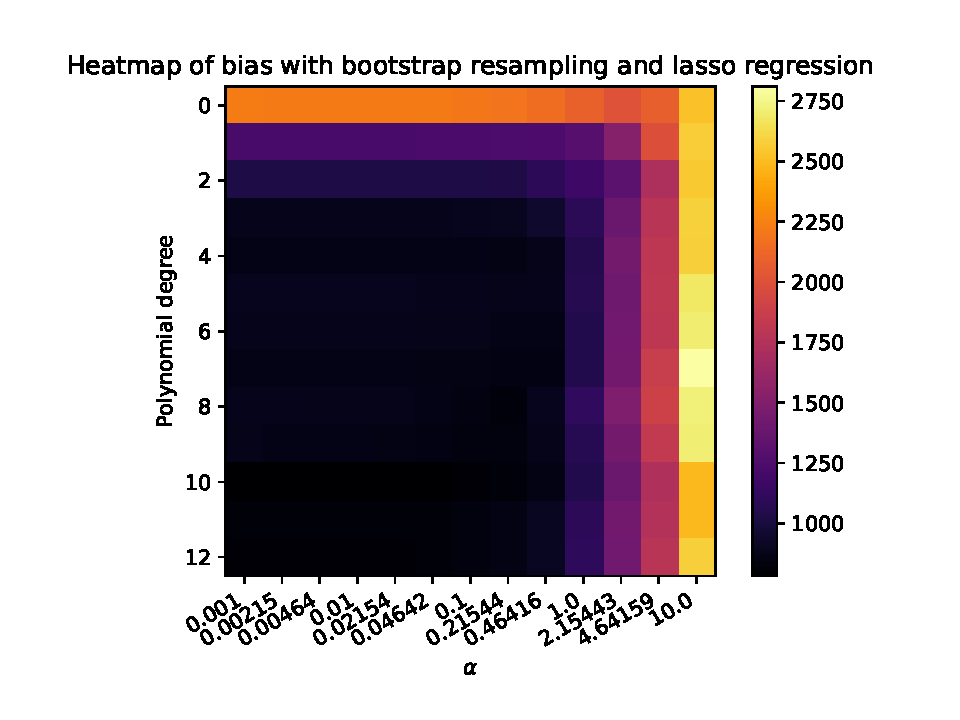
\includegraphics[width=0.45\textwidth]{Heatmap_Bias_Bootstrap_Lasso_Real.pdf} }}%
    \qquad
    \subfloat{{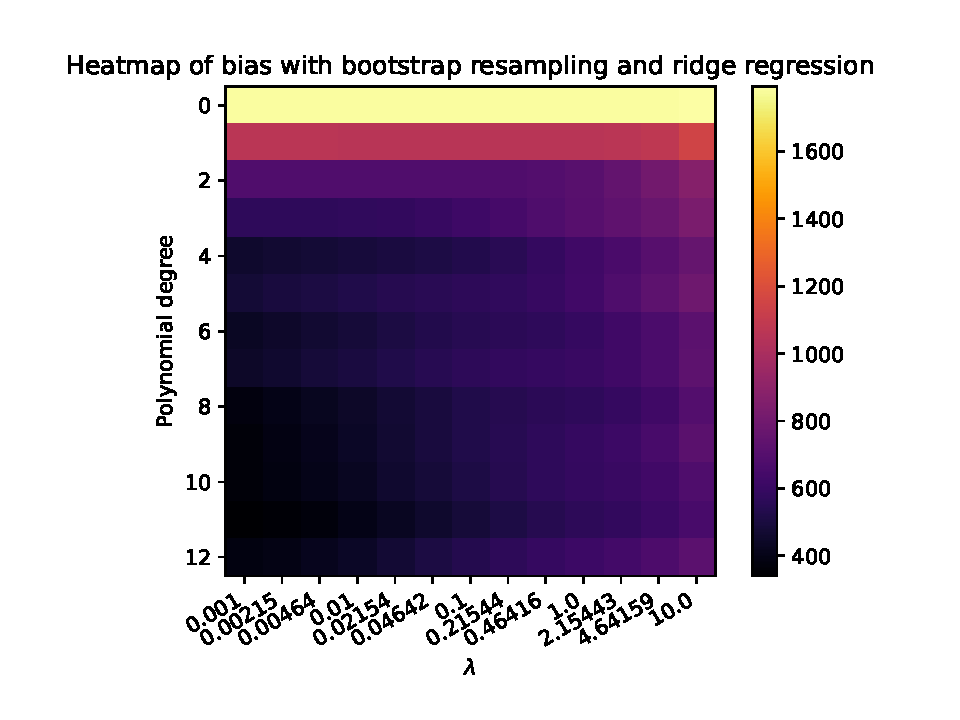
\includegraphics[width=0.45\textwidth]{Heatmap_Bias_Bootstrap_Ridge_Real.pdf} }}%
    \caption{Figures showing the heatmap of the bias when changing the number of polynomials, the values of $\alpha$ in Lasso regression and the values of $\lambda$ in Ridge regression for bootstrapping. The left pictures are from Lasso regression and right are from Ridge, where top is our synthetic data and bottom is the real data.}
    \label{fig:BIAS_BOOT}
\end{figure*}

\begin{figure*}
    \centering
    \subfloat{{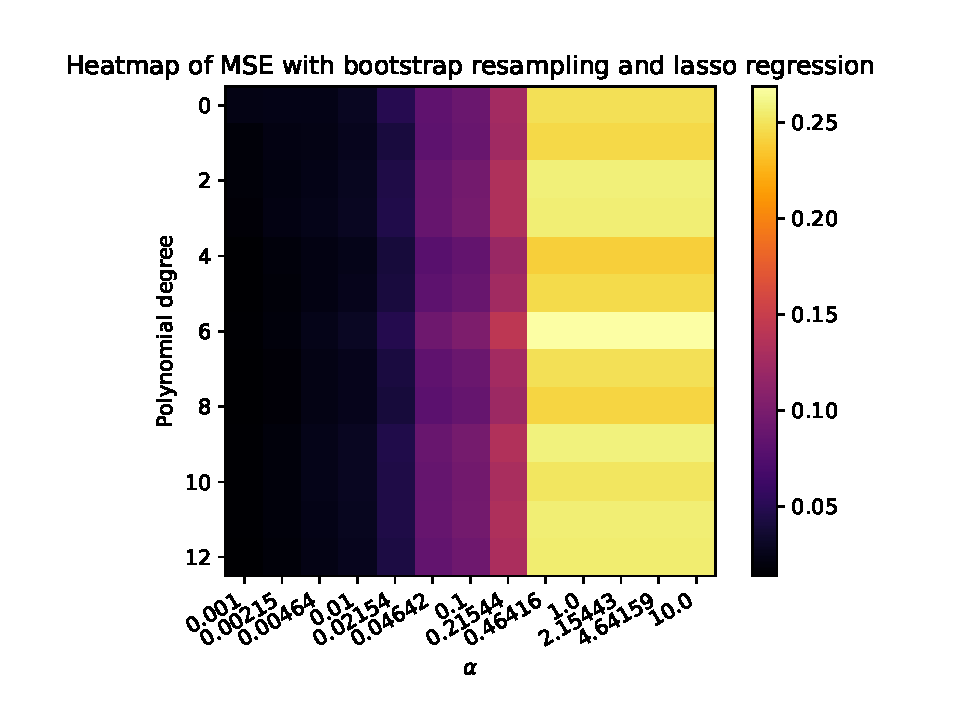
\includegraphics[width=0.45\textwidth]{Heatmap_MSE_Bootstrap_Lasso.pdf} }}%
    \qquad
    \subfloat{{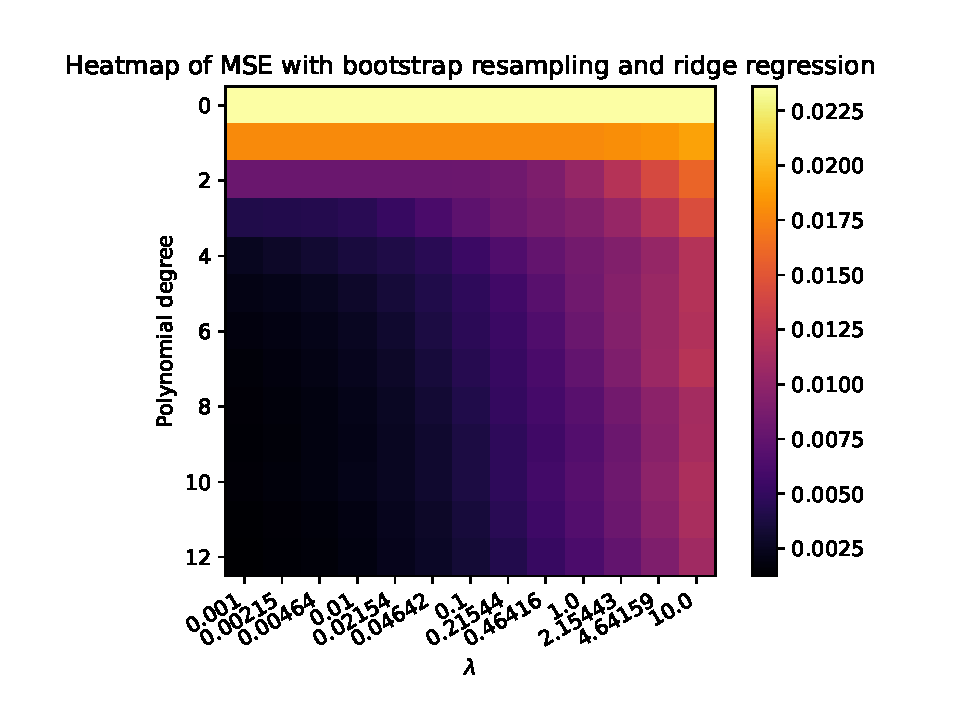
\includegraphics[width=0.45\textwidth]{Heatmap_MSE_Bootstrap_Ridge.pdf} }}%
    \subfloat{{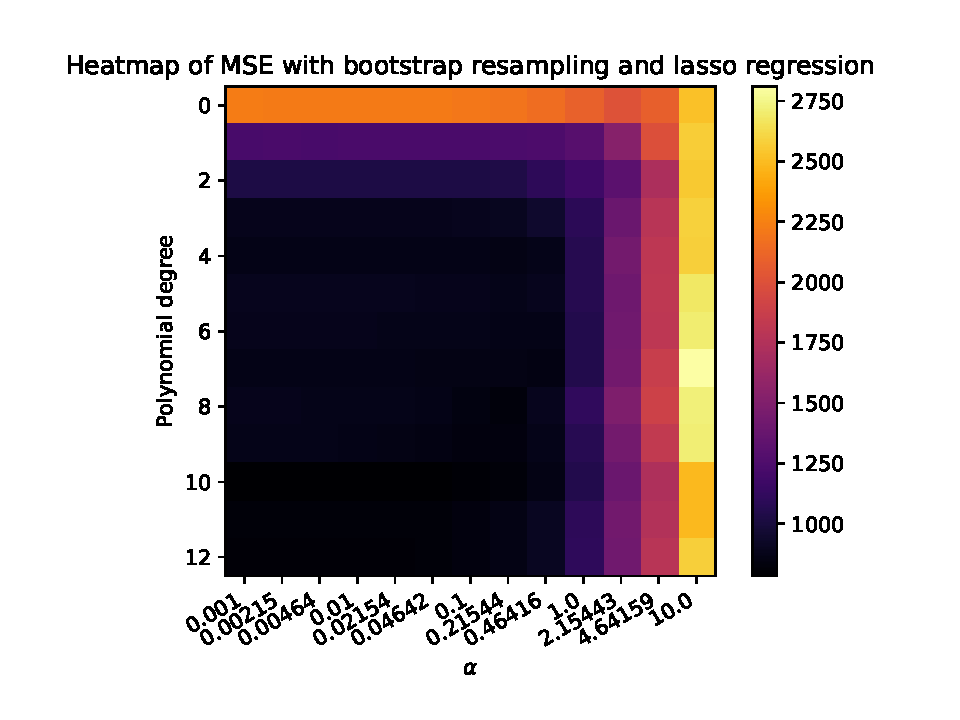
\includegraphics[width=0.45\textwidth]{Heatmap_MSE_Bootstrap_Lasso_Real.pdf} }}%
    \qquad
    \subfloat{{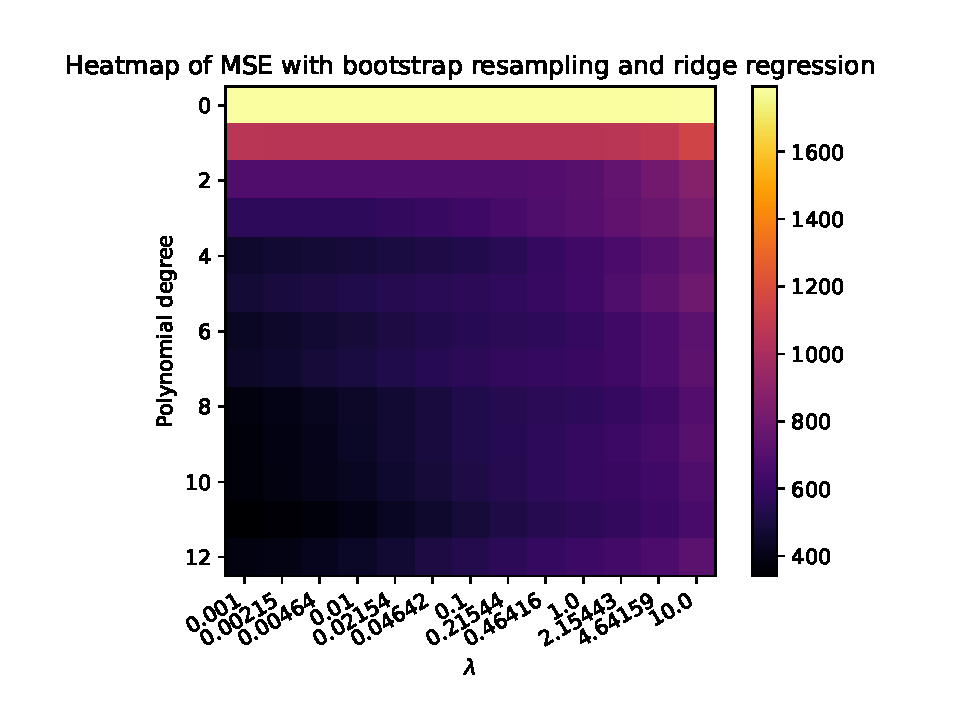
\includegraphics[width=0.45\textwidth]{Heatmap_MSE_Bootstrap_Ridge_Real.pdf} }}%
    \caption{Figures showing the heatmap of the MSE when changing the number of polynomials, the values of $\alpha$ in Lasso regression and the values of $\lambda$ in Ridge regression for bootstrapping. The left pictures are from Lasso regression and right are from Ridge, where top is our synthetic data and bottom is the real data.}
    \label{fig:MSE_BOOT}
\end{figure*}

\begin{figure*}
    \centering
    \subfloat{{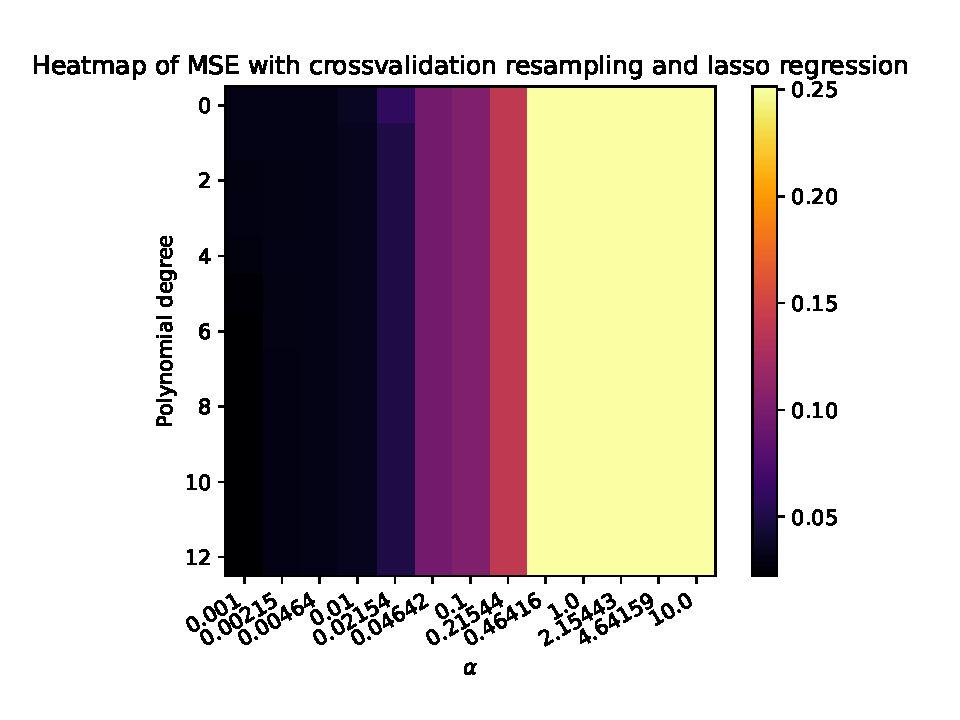
\includegraphics[width=0.45\textwidth]{Heatmap_MSE_Crossvalidation_Lasso.pdf} }}%
    \qquad
    \subfloat{{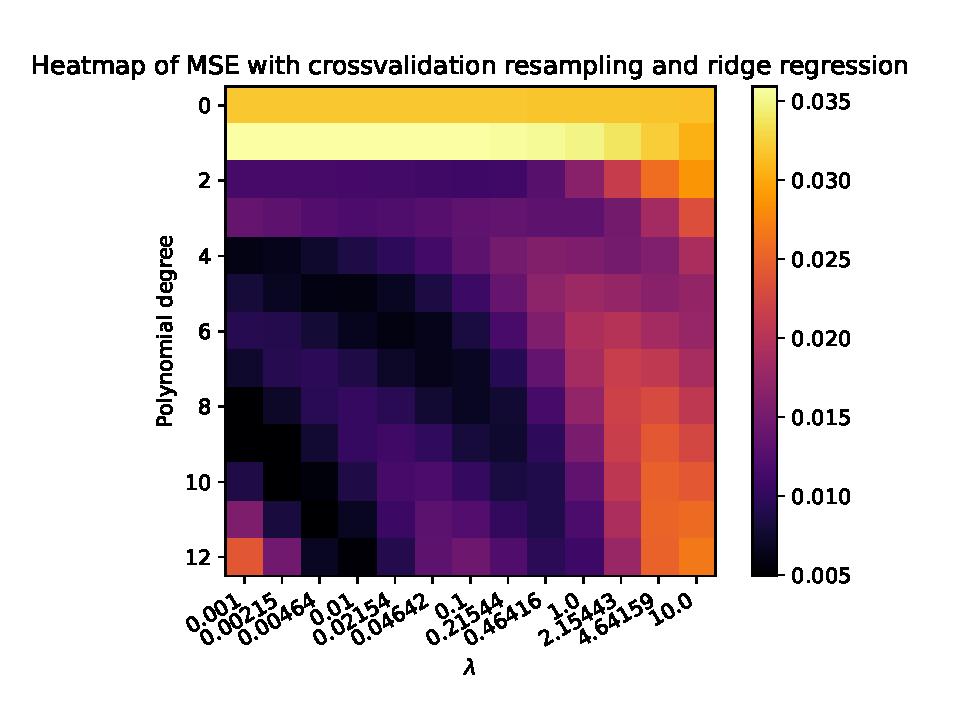
\includegraphics[width=0.45\textwidth]{Heatmap_MSE_Crossvalidation_Ridge.pdf} }}%
    \subfloat{{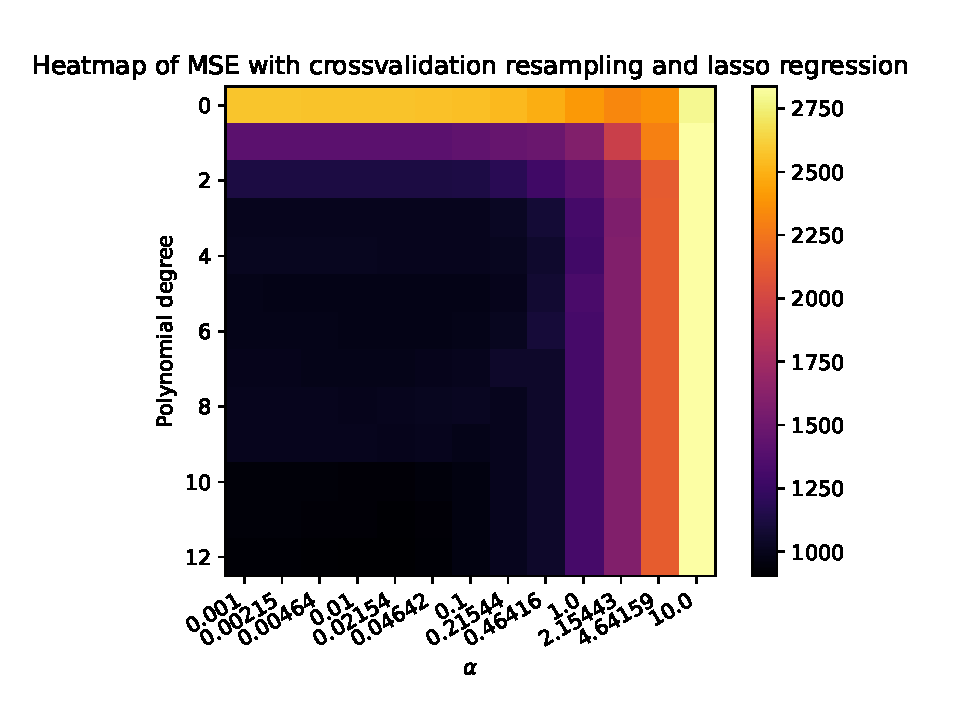
\includegraphics[width=0.45\textwidth]{Heatmap_MSE_Crossvalidation_Lasso_Real.pdf} }}%
    \qquad
    \subfloat{{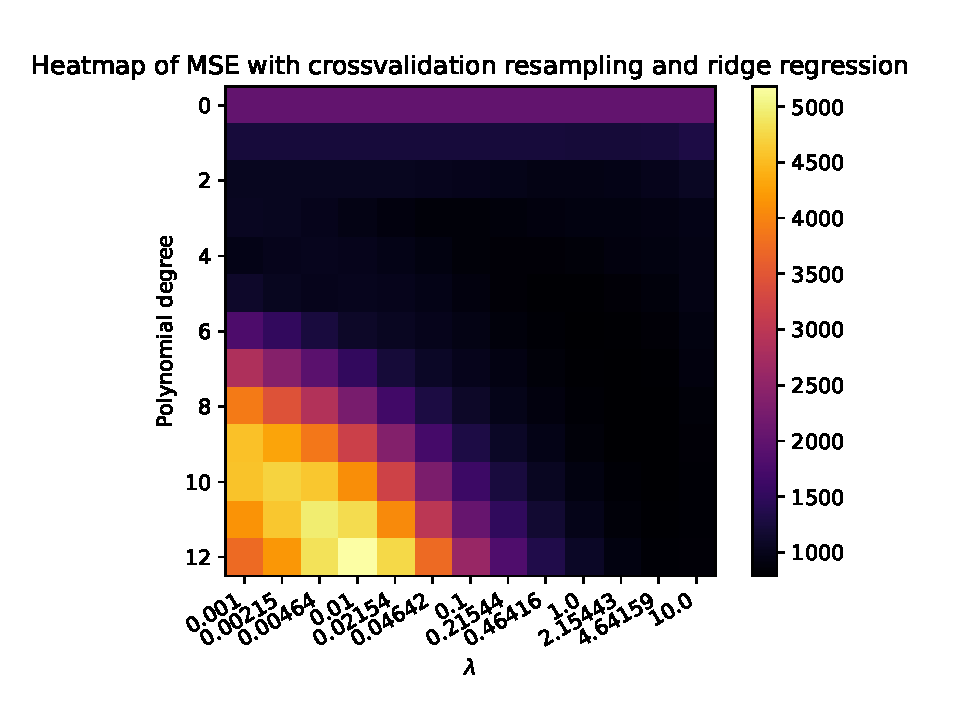
\includegraphics[width=0.45\textwidth]{Heatmap_MSE_Crossvalidation_Ridge_Real.pdf} }}%
    \caption{Figures showing the heatmap of the MSE when changing the number of polynomials, the values of $\alpha$ in Lasso regression and the values of $\lambda$ in Ridge regression for crossvalidation. The left pictures are from Lasso regression and right are from Ridge, where top is our synthetic data and bottom is the real data.}
    \label{fig:MSE_CROSS}
\end{figure*}

\begin{figure*}
    \centering
    \subfloat{{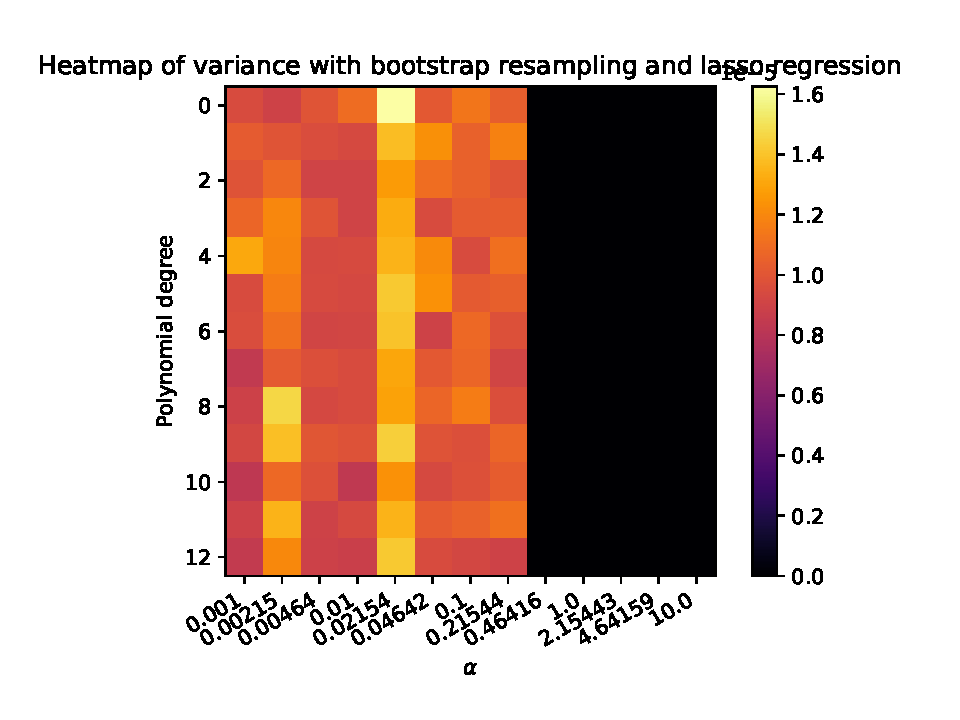
\includegraphics[width=0.45\textwidth]{Heatmap_Variance_Bootstrap_Lasso.pdf} }}%
    \qquad
    \subfloat{{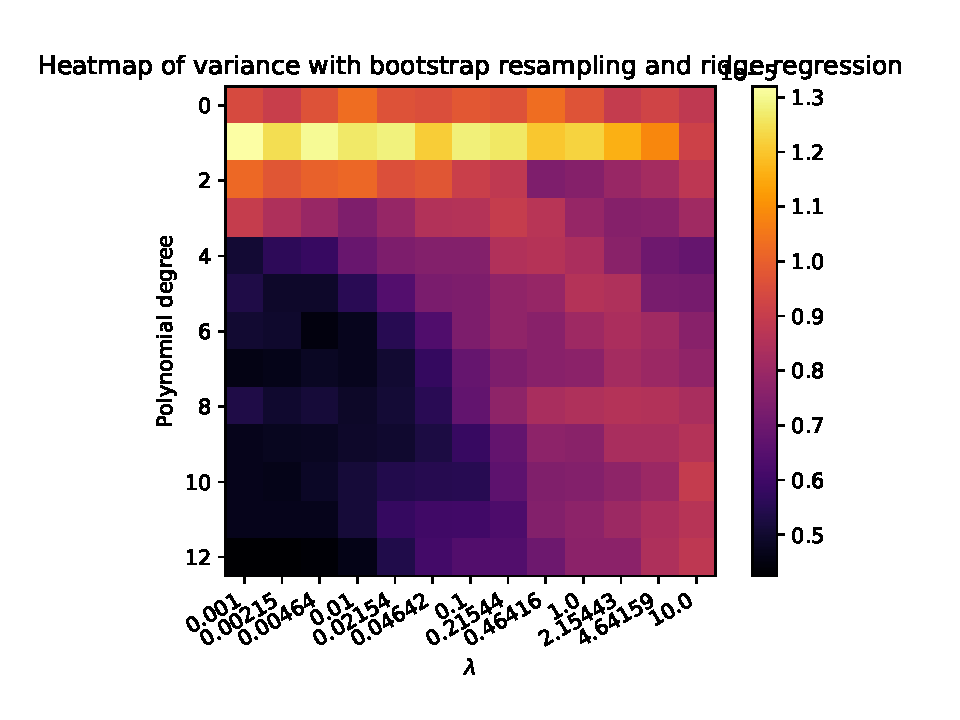
\includegraphics[width=0.45\textwidth]{Heatmap_Variance_Bootstrap_Ridge.pdf} }}%
    \subfloat{{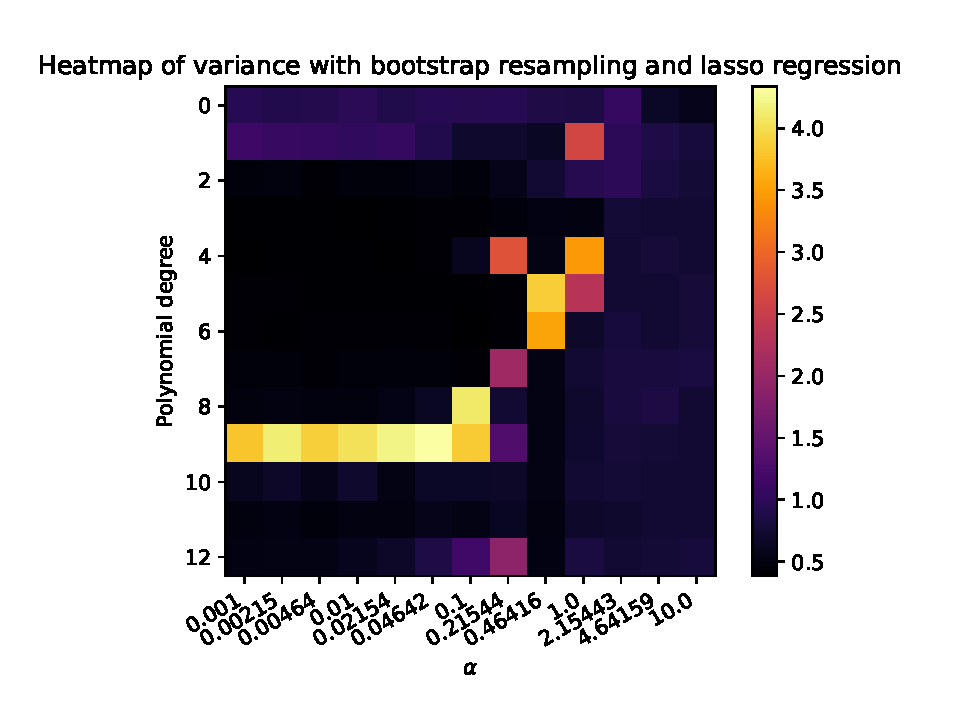
\includegraphics[width=0.45\textwidth]{Heatmap_Variance_Bootstrap_Lasso_Real.pdf} }}%
    \qquad
    \subfloat{{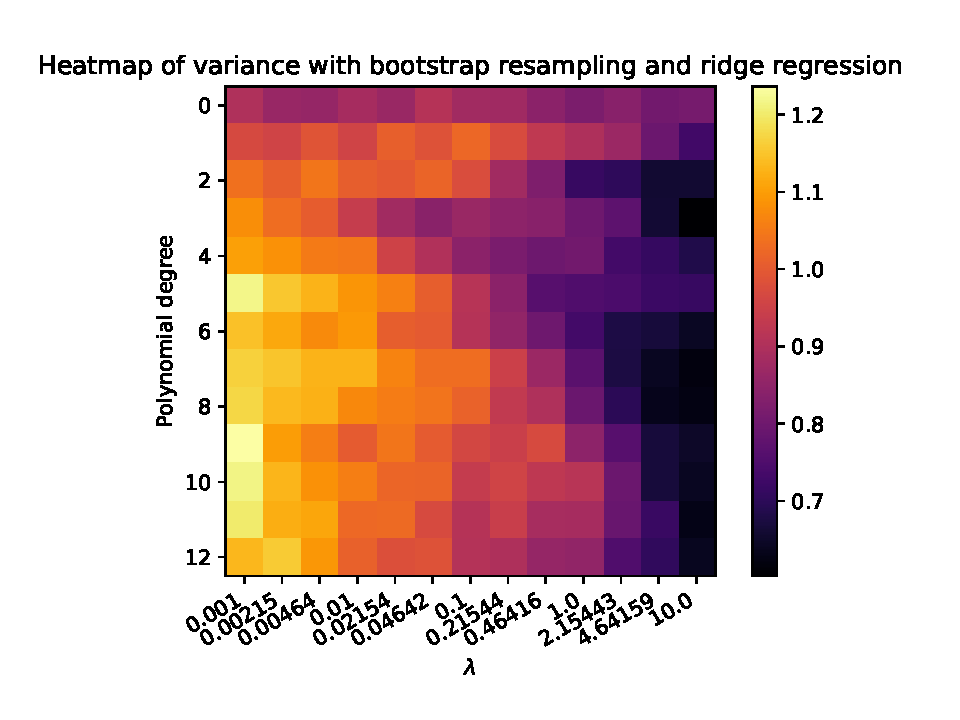
\includegraphics[width=0.45\textwidth]{Heatmap_Variance_Bootstrap_Ridge_Real.pdf} }}%
    \caption{Figures showing the heatmap of the variance when changing the number of polynomials, the values of $\alpha$ in Lasso regression and the values of $\lambda$ in Ridge regression for bootstrapping. The left pictures are from Lasso regression and right are from Ridge, where top is our synthetic data and bottom is the real data.}
    \label{fig:VAR_BOOT}
\end{figure*}


\clearpage

\section{DISCUSSION}\label{sec:DISCUSSION}

As we see in figure (\ref{fig: MSE}), our MSE gradually drops down from $0.3$ to under $0.1$, close to $0$, when changing number of polynomials from one to five, and the $R^2$ score goes from $0.7$ to above $0.9$, very close to $1$. This shows us that our OLS implementation drastically improves when we increase the number of polynomials. It is also interesting to see how similar the test and training data perform, both when looking at the MSE and $R^2$ score. This at least tells us that our algorithm does not over-fit, and is a good indication that we have a generalized solution. Furthermore, when looking at the MSE and $R^2$ score of the real life data, we see the same trend, just that the MSE stops at around $0.1$ and the $R^2$ score at around $0.9$. This indicates that our algorithm is well suited also for real life data, since the data here is not strictly between $0$ and $1$, but can vary between $1107$ and $1530$ (we found this by calculating the min and max value of the sample we used), which means an MSE of $0.1$ is acceptable.
\\
\\
% Dette blir kanskje litt vel mye teori?
%Synes det var bra skrevet, ikke for mye teori etter min mening! :)%
Another indication of whether or not our algorithm is over-fitting can be found by analysing our $\beta$ values. Looking at figure 2, we see that the $\beta$ values in our synthetic data seem to follow a trend between polynomials one to three, with relatively minor changes between the different polynomial degrees. Polynomials four and five, however, have large spikes in their values, meaning that another pathway through the datapoints have been found. This essentially means that a new function, which provides a lower MSE, has been found. This could be due to over-fitting, that our algorithm forces the function to pass through all the data points, rather than following their general trend. It does, however, look as if the $\beta$ values from polynomial degrees four and five also follow a somewhat similar trend. There are deviations between them, but these may be caused by noise. Therefore, instead of being a sign of over-fitting, this could indicate that the new function gives a better explanation of the data. 
The $\beta$ values from our real data behaves similarly, with the first three polynomial degrees showing a clear trend, while polynomial degrees four and five deviate quite a lot from the previous. Polynomial degree five shows some rather large jumps in value compared to polynomial degree four. Looking at this plot alone, one would think that we have entered the realm of over-fitting with polynomial degree five, but, as we suspect with the synthetic data, this could actually be the better function, as we are dealing with quite complex data. Plotting $\beta$ values from higher polynomial degrees could give us better answers, but as the amount of $\beta$s increase more and more for each polynomial degree, the plots would likely be messy and hard to read. 
\\
\\
When further investigating the change in MSE using OLS as seen in figure (\ref{fig: MSE}), we see a clear spike at around $12$ polynomials for the synthetic data, but also a small one for the real data. Our simulated data tells us that the best number of polynomials is 10, and the real data seems to confirm this aswell, with an MSE as low as $0.01$ for both. This proves to us that there is an optimal amount of polynomials, and that adding more polynomial degrees will give us worse results.
\\
\\
Using what we now know about our OLS, we want to test the same for our simple bootstrapping method, and compare the results. Looking at figure (\ref{fig: BOOTSTRAP}), we see that the bootstrapping method results in a much lower MSE for our synthetic data. The MSE also does not spike at around 12 polynomials, but seems to be stable, indicating that it might be able to handle more polynomials and perform better. However, we see that bootstrapping for our real data gave worse results than simply using OLS as discussed above. A reason for this could be the fact that the real data has larger numbers, and that some of the bootstrap samples end up with one of the few unlucky results giving a large MSE due to this.
\\
We also see in both pictures that the bias is very high when dealing with a low polynomial degree, which means that a low degree of polynomials results in an underfit, which is to be expected. We also see the variance and MSE being low, even when we go up to $18$ polynomials, both for $100$ and $500$ iterations of bootstrapping. This could be due to the fact that we used high numbers of bootstrapps, and if we decreased either this further down than $100$ or increased the number of polynomials we would see an increase in variance and MSE as we do this, because then our model would overfit as we saw happened for $12$ polynomials and up in figure (\ref{fig: MSE}).
\\
\\
As we see in figure (\ref{fig:KFOLD}), the Cross-validation method is a bit worse than bootstrapping. We also see that Cross-validation, both for $5$ and $10$ folds get worse a lot faster when increasing polynomials. Using $5$ polynomials and $10$ folds seems to be about as optimal of a solution from Cross-validation as we can get, but still a lot worse than bootstrapping. However, factoring in the computation speed, an MSE of $0.02$ for our $100 \times 100$ synthetic data is not a bad result. When looking at the real data, we see the MSE being a lot higher, but as stated earlier, the real data uses larger numbers, so the MSE here is also not that unacceptable. Therefore, if we were to deal with larger data sets than this, a simple Cross-validation implementation could prove useful for quick results.
\\
\\
Now when looking at the heatmap figures (\ref{fig:BIAS_BOOT}, \ref{fig:MSE_BOOT}, \ref{fig:MSE_CROSS}, \ref{fig:VAR_BOOT}), we observe firstly how well Lasso and Ridge performs compared to the earlier resampling techniques. When looking at the heatmaps, there are no clear indication whether Ridge or Lasso is a better choice. Ridge seems to in general outperform Lasso to some degree, but using their optimal parameters seems to give very similar result. When looking at the real data however, we see that Ridge slightly outperforms Lasso on MSE and bias when bootstrapping. For variance however, as seen in figure (\ref{fig:VAR_BOOT}), Lasso seems to give better results. This may indicate that Ridge is better at not under-fitting, which means it will also outperform on smaller numbers of polynomials, while Lasso seems to be better at not overfitting. The optimal parameters for Lasso when looking at the real data seems to be an $\alpha$ at around 0, and number of polynomials at around $10$. For Ridge, the optimal parameters seem to be at a $\lambda$ around $0$ (not for variance though, as we see here a $\lambda$ around 10 would be better), and a polynomial degree of about $11$.
\\
However, when looking at figure (\ref{fig:MSE_CROSS}), we see different behaviors. Here the optimal values seem to be different for Ridge, where optimal polynomial degree is about $4$ both for training and real data combined. We also see that the MSE scale is a lot higher on Cross-validation for Ridge than it was on bootstrapping, while Lasso keeps about the same scale. This shows us that Lasso regression is more suited if we need to use a quicker resampling method like Cross-validation. So if we want quick computation, we should choose Lasso with Cross-validation, but if we want a highly precise model with low MSE, we choose Ridge with bootstrapping, but make sure to not use too many polynomials, as we will then overfit.


\section{CONCLUSION}\label{sec:CONCLUSION}
    So to summarize, we have now tested our model and found the capabilities of OLS with regards to where OLS overfits and underfits, but also how small of an MSE we can achieve. We also saw how implementing bootstrapping helped decrease the MSE drastically, while also drastically reducing the rate in which our model overfits. We saw that Cross-validation was indeed outperformed, but did provide pretty decent results for its computation time. We also saw how Ridge regression outperformed Lasso, but Lasso could be a good alternative combined with for example Cross-validation for a much shorter computation time.
\section{CODE}\label{sec:CODE}
The code used to simulate can be found at \href{https://github.com/mathiasmellemstuen/FYS-STK4155-Prosjekt-1}{this} Github repository.

\appendix

\section{Numerical Notation}\label{sec:NOTATION}

X = \begin{bmatrix}
1 & x_0^1 & x_0^2 & ... & ... & x_0^{n-1}\\
1 & x_1^1 & x_1^2 & ... & ... & x_1^{n-1}\\
1 & x_2^1 & x_2^2 & ... & ... & x_2^{n-1}\\
... & ... & ... & ... & ... & ... \\
1 & x_{n-1}^1 & x_{n-1}^2 & ... & ... & x_{n-1}^{n-1}
\end{bmatrix}

\begin{align*}\label{eq:E_y}
    y_i &= \beta_0 x_{i0} + \beta_1 x_{i1} + ... + \beta_n-1 x_{in-1} + \epsilon_i \\
    &= \sum_j x_{ij} \beta_j + \epsilon_i \\
    \mathbb{E}(y_{i}) &=  \mathbb{E}(\sum_j x_{ij} \beta_j + \epsilon_i ) \\
    &= \mathbb{E}(\sum_j x_{ij} \beta_j) + E(\epsilon_i) = \sum_j \mathbb{E}(x_{ij} \beta_j) + 0 \\
    &= \sum_j x_{ij} \beta_j = X_{i,*}\beta 
\end{align*}


\begin{align*}\label{eq:var_y}
    Var(y_{i}) &= \mathbb{E}((y_{i} - \bar{y_{i}})^2) = \mathbb{E}((y_{i} - \mathbb{E}(y_{i}))^2) \\
    &= \mathbb{E}(y_{i}^2) - 2\mathbb{E}(y_{i})\mathbb{E}(y_{i}) + (\mathbb{E}(y_{i}))^2 \\ 
    &= \mathbb{E}(y_{i}^2) - (\mathbb{E}(y_{i}))^2 = \mathbb{E}((X_{i,*}\beta + \epsilon)^2) - (X_{i,*}\beta)^2 \\ 
    &= \mathbb{E}((X_{i,*}\beta)^2 + 2\epsilon_{i} X_{i,*}\beta + \epsilon_{i}^2) - (X_{i,*}\beta)^2 \\ 
    &= (X_{i,*}\beta)^2 + 2\mathbb{E}(\epsilon_{i})X_{i,*}\beta + \mathbb{E}(\epsilon_{i}^2) - (X_{i,*}\beta)^2 \\
    &= \mathbb{E}(\epsilon_{i}^2) = Var(\epsilon_{i}) = \sigma^2
\end{align*}

\begin{align*}\label{eq:E_beta}
    \mathbb{E}(\hat{\beta}) &= \mathbb{E}(X^TX)^{-1}X^Ty) = (X^TX)^{-1}X^T\mathbb{E}(y) \\&= (X^TX)^{-1}X^TX\beta = \beta
\end{align*}

\begin{align*}\label{eq:var_beta}
    Var(\hat{\beta}) &= \mathbb{E} [(\beta - \mathbb{E}(\beta))(\beta - \mathbb{E}(\beta))^T] \\
    &= \mathbb{E}[((X^T X)^{-1} X^T Y - \beta) ((X^T X)^{-1} X^T Y - \beta)^T] \\
    &= (X^T X)^{-1} \mathbb{E}(Y Y^T) X (X^T X)^{-1} - \beta \beta^T \\
    &= \beta \beta^T + \sigma^2 (X^T X)^{-1} - \beta \beta^T = \sigma^2 (X^T X)^{-1}
\end{align*}
\\

\begin{align*}\label{eq:BIAS_VAR}
    C(\mathbf{X}, \mathbf{\beta}) &= \frac{1}{n} \sum_{i = 0}^{n - 1} (y_i - \tilde y_i)^2 = \mathbb{E}[(\textbf{y} - \mathbf{\tilde y})^2] \\
    \mathbb{E}[(\textbf{y} - \mathbf{\tilde y})^2] &=  \frac{1}{n} \sum_{i = 0}^{n - 1} (f_i - \mathbb{E}[\tilde y_i])^2 + \frac{1}{n} \sum_{i = 0}^{n - 1} (\tilde y_i - \mathbb{E}[\tilde y_i])^2 + \sigma^2 \\
    \mathbb{E}[(\textbf{y} - \mathbf{\tilde y})^2] &= \mathbb{E}[(\mathbf{f} + \mathbf{\epsilon} - \mathbf{\tilde y})^2] = \mathbb{E}[(\mathbf{f} + \mathbf{\epsilon} - \mathbf{\tilde y} + \mathbb{E}[\mathbf{\tilde y}] - \mathbb{E}[\mathbf{\tilde y}])^2] \\
    &= \mathbb{E}[(\textbf{y} - \mathbb{E}[\mathbf{\tilde y}])^2] + Var[\mathbf{\tilde y}] + \sigma^2
\end{align*}


\section{Functions}\label{sec:FUNCTIONS}

\begin{align*}\label{eq:FrankeFunction}
    f(x,y) &= \frac{3}{4} exp \left( \frac{(9x -2)^2}{4} - \frac{(9y -2)^2}{4}  \right) \\
    &+  \frac{3}{4} exp \left( -\frac{(9x + 1)^2}{49} - \frac{(9y + 1)}{10} \right) \\
    &+ \frac{1}{2} exp \left( -\frac{(9x -7)^2}{4} - \frac{(9y - 3)^2}{4} \right) \\
    &- \frac{1}{5} exp \left( - (9x - 4)^2 - (9y - 7)^2 \right)
\end{align*}
\end{document}